\begin{frame}{Right Triangle with Measurements}
\begin{center}
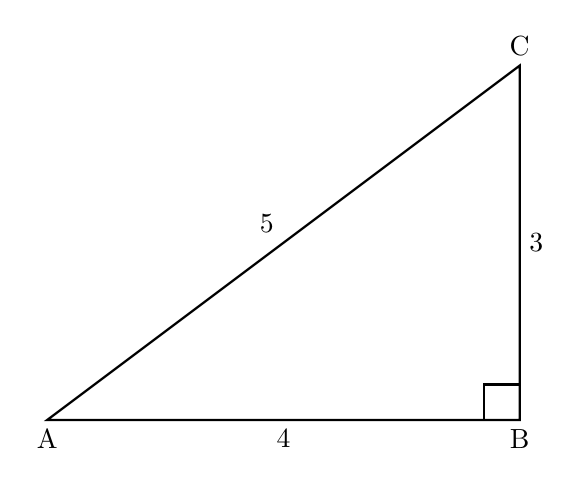
\begin{tikzpicture}[scale=1.5]
    \draw[thick] (0,0) -- (4,0) -- (4,3) -- cycle;
    \node[below] at (0,0) {A};
    \node[below] at (4,0) {B};
    \node[above] at (4,3) {C};
    
    % Right angle mark
    \draw[thick] (3.7,0) -- (3.7,0.3) -- (4,0.3);
    
    % Side lengths
    \node[below] at (2,0) {4};
    \node[right] at (4,1.5) {3};
    \node[above left] at (2,1.5) {5};
\end{tikzpicture}
\end{center}

\footnotesize
\texttt{\textbackslash draw[thick] (3.7,0) -- (3.7,0.3) -- (4,0.3);}
\end{frame}